\documentclass{article}

\usepackage{graphicx}
\usepackage{hyperref}
\usepackage{amsmath}

\graphicspath{{../images/}}

\begin{document}

\section{H-1.1}

One signal point can represent 2 bits. The constellation can be seen in \autoref{fig:4qam}.
\begin{figure}[h]
\centering
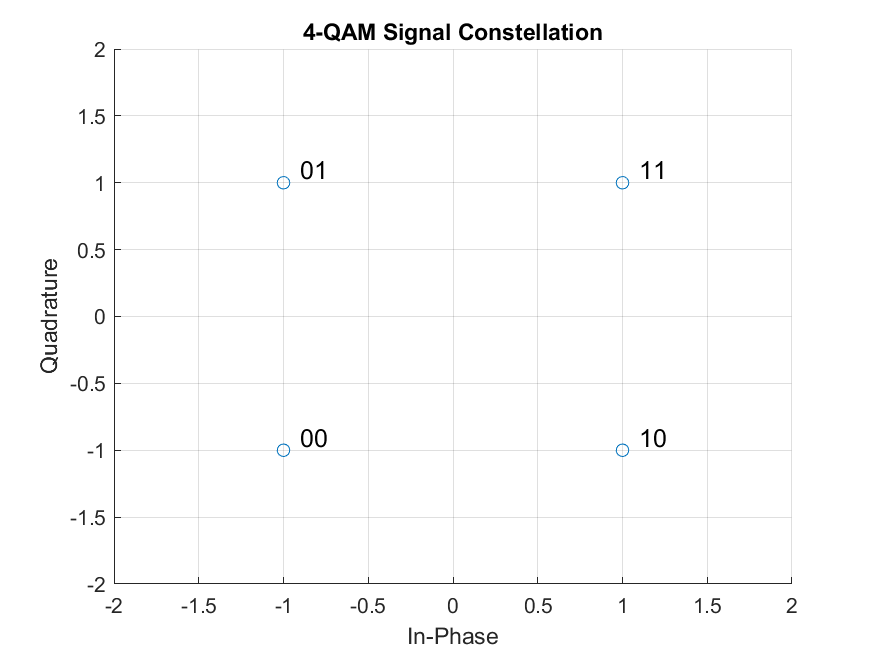
\includegraphics[width=\textwidth]{4_QAM.png}
\caption{4-QAM constellation}
\label{fig:4qam}
\end{figure}

\section{H-1.2}

The X-Y mode plots 2 signals against each other. So for example the in-phase and quadrature signals.

\section{H-1.3}

\begin{equation}
\textrm{PAPR} = \frac{max_m\{P_m\}}{E\{P_m\}}
\end{equation}

\begin{equation}
P_m = \Re{(m)}^2 + \Im{(m)}^2
\end{equation}
\subsection{2ASK}
\subsubsection{unipolar}

\begin{equation}
\textrm{PAPR} = \frac{1^2}{\frac{1}{2}(1^2+\frac{1}{2}^2)} = \frac{1}{\frac{1}{2}\frac{5}{4}} = \frac{8}{5}
\end{equation}

\subsubsection{bipolar}

\begin{equation}
\textrm{PAPR} = \frac{1^2}{\frac{1}{2}(1+1)} = 1
\end{equation}

\subsection{8ASK}
\subsubsection{unipolar}

\begin{flalign}
\textrm{PAPR} &= \frac{1^2}{\frac{1}{8}(1^2+\frac{7}{8}^2+\frac{6}{8}^2+\frac{5}{8}^2+\frac{4}{8}^2+\frac{3}{8}^2+\frac{2}{8}^2+\frac{1}{8}^2)} &&\\\nonumber
&=\frac{1}{\frac{1}{8}\frac{51}{16}} &&\\\nonumber
&=\frac{128}{51} \approx 2.5098 &&
\end{flalign}

\subsubsection{bipolar}

\begin{flalign}
\textrm{PAPR} &= \frac{1^2}{\frac{1}{8}((-1)^2+(-\frac{5}{7})^2+(-\frac{3}{7})^2+(-\frac{1}{7}^2+\frac{1}{7}^2+\frac{3}{7}^2+\frac{5}{7}^2+1^2)} &&\\\nonumber
&=\frac{1}{\frac{1}{8}\frac{10617}{3136}} &&\\\nonumber
&=\frac{25088}{10617} \approx 2.363 &&
\end{flalign}

\subsection{16QAM}

Power of corner points is:
\begin{equation}
P_{corner} = 1^2 + 1^2 = 2
\end{equation}

Power of outer middle points is:
\begin{equation}
P_{outermiddle} = \frac{1}{3}^2 + 1^2 = \frac{10}{9}
\end{equation}

Power of inner points is:
\begin{equation}
P_{inner} = \frac{1}{3}^2 + \frac{1}{3}^2 = \frac{2}{9}
\end{equation}

So the PAPR is:
\begin{flalign}
\textrm{PAPR} &= \frac{2}{\frac{1}{16}(4*2 + 8*\frac{10}{9} + 4*\frac{2}{9})} &&\\\nonumber
&=\frac{2}{\frac{1}{16}\frac{160}{9}} &&\\\nonumber
&=\frac{9}{5} = 1.8 &&
\end{flalign}

\subsection{8PSK}
For 8PSK the Power for all points is 1 (all on unit circle).
\begin{flalign}
\textrm{PAPR} &= \frac{1}{\frac{1}{8}(8*1)} &&\\\nonumber
&=\frac{1}{1} = 1 &&
\end{flalign}

\subsection{Crest Factor}
The crest factor is just the maximum amplitude divided by the RMS of the amplitude.
So it is the same as PAPR, only calculated for the amplitude, not the power.
Thus when expressed in decibels, crest factor and PAPR are equivalent.

\section{H-1.4}
The radio-frequency signal is used to upconvert the baseband signal to around the carrier frequency.
So when they are added they create the modulated signal.

\section{H-1.5}
The optimal filter is the matched filter.
It's optimization criterion is to maximize the signal to noise ratio.

\begin{equation}
h(kT_s) = \begin{cases} 1; & k = 0 \\ 0; & k \neq 0 \end{cases}
\end{equation}
\begin{equation}
\frac{1}{T_s} \sum_{k = -\infty}^{+\infty} H \left( f - \frac{k}{T_s} \right) = 1
\end{equation}

In \autoref{fig:sinc} the function $sinc(x)$ is shown.
It is 1 for $k = 0$ and 0 for all other values as is necessary for the time criterion.

\begin{figure}[h]
\centering
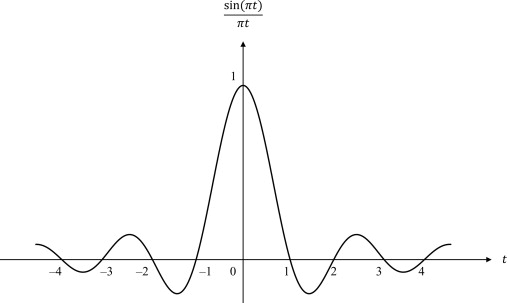
\includegraphics[width=\textwidth]{sinc.jpg}
\caption{Sinc function}
\label{fig:sinc}
\end{figure}

The rectangular function seen in \autoref{fig:rect} is the fourier transform of the sinc function.
One can sum up the area under the function to get 1, as the frequency criterion requires.

\begin{figure}[h]
\centering
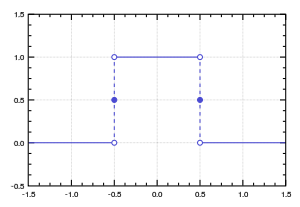
\includegraphics[width=\textwidth]{rect.svg.png}
\caption{rect function}
\label{fig:rect}
\end{figure}

\section{H-1.6}
By minimizing the variation of the envelope of the signal the crest factor is minimized.
This helps with power efficiency.
And there is less back-off for the power amplifier at the transmitter necessary. (from lecture p.92, slide 163)
\end{document}
